\documentclass{beamer}

% Define theme (optional)
\usetheme{default}

% Packages for math symbols and equations
\usepackage{amsmath}
\usepackage{amsfonts}
\usepackage{amssymb}

% For including images
\usepackage{graphicx}
\graphicspath{{../imgs/}}

% Additional packages
\usepackage{hyperref} % For hyperlinks
\usepackage{tikz} % For diagrams
\usepackage{caption} % For customizing captions
\usepackage{enumitem} % For customizing lists
\usepackage{xcolor} % For defining colors
\usepackage{pgfplots} % For plots and graphs

% Title page information
\title{Air pump fault / anomaly detection}
\author{Antonín Hruška}
\date{\today}

\begin{document}

\begin{frame}
    \titlepage
\end{frame}

\begin{frame}{Task definition}
    \framesubtitle{What we want?}
    
    % Two-column layout
    \begin{columns}[T]
        \small
        % Column 1: Formal definition
        \begin{column}{0.5\textwidth}
            \textbf{Formal Definition:}
            \begin{itemize}
                \item \textbf{Task:}  Fault detection / isolation (offline)
                \item \textbf{Objective:} An (optimal) classifier $h: \mathbb{R}^n  \to \{0, 1\}$ to predict fault occurrence
                \item Supervised classification on time series 
            \end{itemize}
        \end{column}
        
        % Column 2: Informal description
        \begin{column}{0.5\textwidth}
            \textbf{Informal Description:}
            \begin{itemize}
                \item Pump broke / pinpoint its cause (after it happend)
                \item A system that examines a time series of measurments and determines if a specific fault happend
                \item We have labeled data (even those, were fault occured) 
            \end{itemize}
        \end{column}
    \end{columns}

    % Math equations
    \begin{itemize}
        \item Dataset $ \mathcal{D}_{\mathcal T} = \big\{ (\{x_1, x_2, ..., x_{n^i}\},y^i) |\,i \in \{1,...,m\} \big\}$.
    \end{itemize}
    

\end{frame}


\begin{frame}{Theoretical background and our knowledge}
    \framesubtitle{What we know?}
    
    \begin{itemize}
        \item Fault / anomaly detection:
        \begin{itemize}
            \item Traditionaly we have only working model $p_{\text{working}}(\boldsymbol{x})$
            \item Anomalies are measurments highly unlikely under the model.
        \end{itemize}
        
        \item Fault isolation approach:
            \begin{itemize}
                \item Assumes models for both: $p_{\text{working}}(\boldsymbol{x})$ and $p_{\text{faulty}}(\boldsymbol{x})$
                \item Based on hypothesis testing and likelihood ratio tests, i.e. 
                $$\log(p_{\text{working}}(\boldsymbol{x})) - \log(p_{\text{faulty}}(\boldsymbol{x})) > \theta$$
            \end{itemize}
        
        \item Exploiting physics and environment:
            \begin{itemize}
                \item Air pump is a dynamical system. Use shadow box modelling (State space based on physics, Kalman filter) or use data driven methods (Min Squares, ARMA)
                \item We would need more details about measurments, the air pump architecture, the enviroment and the reference signal.
            \end{itemize}
    \end{itemize}
\end{frame}


\begin{frame}{Model}
    % Describe your model here
    \begin{itemize}
        \item Simplistic generative model based on heuristics and examination of the time series.
        \item Naive Bayes Gaussian classifier on first quarter of trimmed sequence.
    \end{itemize}
    \begin{align*}
    p_{\text{working}}(\boldsymbol{x}) = \pi_{\text{working}} \prod_{j=1}^{n_i}p(x_j| \text{working}) \\
    p_{\text{faulty}}(\boldsymbol{x}) =  \pi_{\text{faulty}} \prod_{j=1}^{n_i}p(x_j| \text{faulty}) 
    \end{align*}
\end{frame}

\begin{frame}
    % Add image
    \begin{figure}
        \centering
        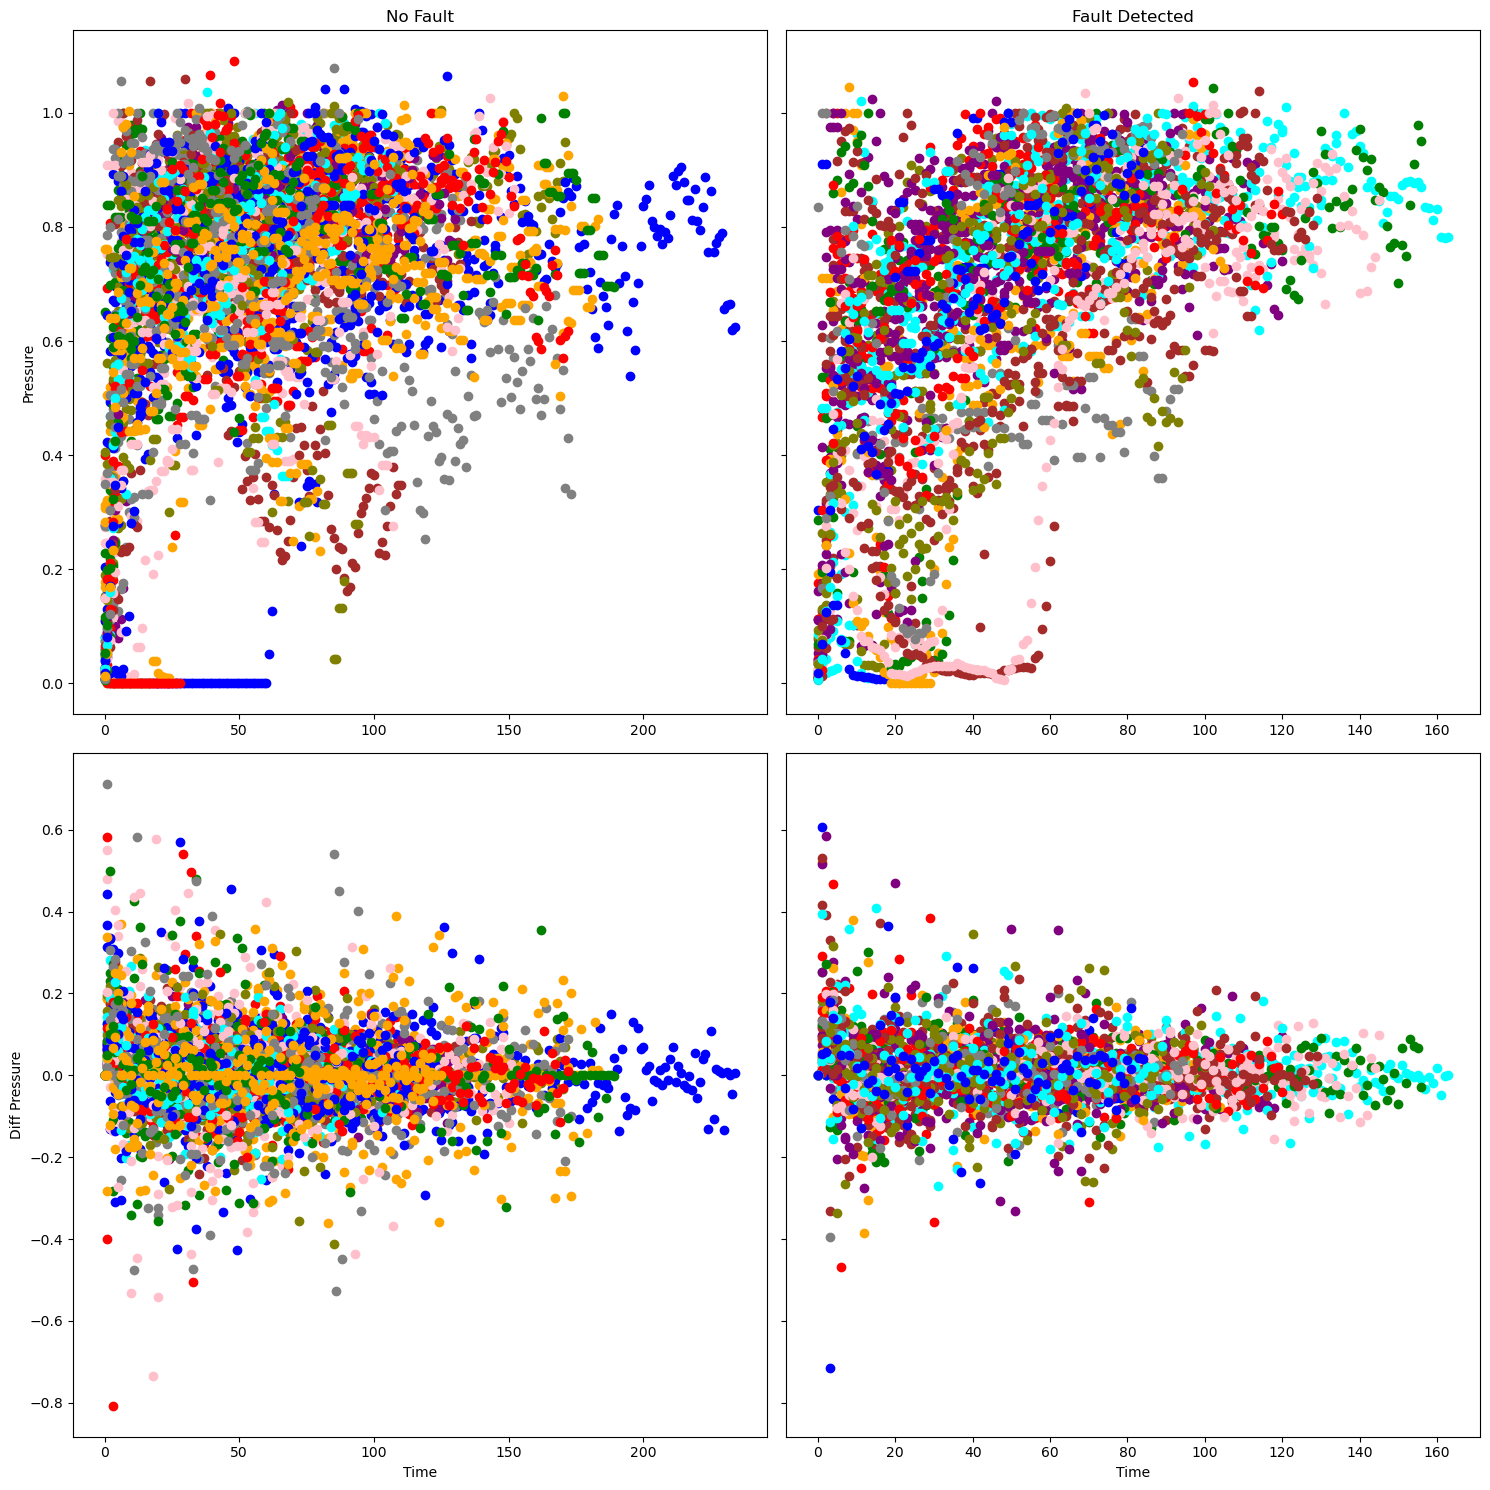
\includegraphics[width=0.67\linewidth]{more_all_faults_only_half.png}
        \caption{ \footnotesize Trimmed sequences with min-max normalization. Upper row: Pressure, Lower row: Pressure difference. Left column: Regular, Right column: Faulty.}
    \end{figure}
\end{frame}


\begin{frame}{Results and future work}
    % Discuss potential future work or proposals here
    \begin{table}[h]
        \centering
        \begin{tabular}{|l|c|c|}
        \hline
        \multicolumn{1}{|c|}{\textbf{}}                & \multicolumn{1}{l|}{\textbf{Actual Positive}} & \multicolumn{1}{l|}{\textbf{Actual Negative}} \\ \hline
        \multicolumn{1}{|l|}{\textbf{Predicted Positive}} & 445                                            & 1245                                          \\ \hline
        \multicolumn{1}{|l|}{\textbf{Predicted Negative}} & 128                                            & 3562                                          \\ \hline
        \end{tabular}
        \caption{Confusion Matrix (All predictions: 5380, Accuracy 0.74)  on random split of 0.7 trn / 0.2 val / 0.1 test (one run only)}
        \end{table}
    \begin{itemize}
        \item Try more complex model with knowledge of dynamical system and physics.
        \item Or use very simple Deep Learning or Random Forest and hope for strong regularization.
    \end{itemize}
\end{frame}

\end{document}
